\chapter{Literature Review}

\section{Associative Memory}
Associative memory also known as content addressable was first proposed in the
early 1960s by researchers at IBM, including Richard W. Harker, Kenneth C.
Thompson, and Robert D. Denny. CAM is a type of computer memory that allows for
the rapid searching and retrieval of data by using the content of the data as
the address.

In traditional random access memory (RAM), data is stored in a specific
location based on a numerical address, and the data can be retrieved by
accessing the corresponding address. In contrast, CAM stores data in a specific
location based on the content of the data, and the data can be retrieved by
searching for the specific content rather than the numerical address.

CAM has several advantages over traditional RAM, including faster search and
retrieval times and the ability to store and retrieve data based on the content
rather than a numerical address. These features make CAM particularly useful in
applications where rapid searching and retrieval of data is important, such as
database management and pattern recognition.

The concept of CAM has had a significant impact on the field of computer
science. The work of Harker, Thompson, and Denny has contributed to the
development of efficient and effective methods for storing and retrieving data
in computers.Its applications include database management systems which require
searching through the data as fast as possible figure\ref{associative_circuit}
shows one such circuit.
\begin{figure}[h!]
    \centering
    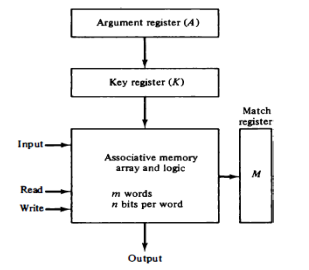
\includegraphics[width=0.7\linewidth]{associative}
    \caption{Associative memory circuit}\label{associative_circuit}
\end{figure}

\section{Associative network}
An associative network is a type of artificial neural network that is designed
to store and retrieve information based on the strength of the connections
between neurons. Associative networks are often used for tasks that require the
recall of specific patterns or relationships, such as image recognition,
natural language processing, and recommendation systems.
\subsection{An Interactive Activation Model of Context Effects in Letter Perception}
\subsubsection{Introduction}
The interactive activation model\cite{auto} is a computational model that
attempts to explain how the brain processes and interprets written language. It
suggests that the brain stores and retrieves information about letters and
words based on the strength of the connections between neurons, and that these
connections are influenced by both bottom-up and top-down processes.

The model proposes that the brain has a hierarchical structure, with
lower-level processing units representing features such as lines and curves,
and higher-level processing units representing letters and words. According to
the model, the activation of a processing unit depends on both the activation
of its inputs and the activation of its outputs.
\subsubsection{Proposed system}
The authors propose a hierarchical structure for the model, with lower-level
processing units representing features such as lines and curves, and
higher-level processing units representing letters and words. They suggest that
the activation of a processing unit depends on both the activation of its
inputs and the activation of its outputs.The main two concept in this ssytem
are
% Neural associative memory is
% also known as the associative network, which works based on pattern
% association. It can store different patterns and produce the output which
% closely matches the already given patterns. They are implemented using the
% artificial neural network, which tries to mimic the working of the brain. They
% are commonly used in applications like pattern recognition, data storage and
% information retrieval. There are two types of associative networks
\begin{description}
    \item[Auto associative memory]A single layer NN in which the number of training
    vectors and the number of output vectors are the same. The weights are
    determined by the stored patterns
    \item[Hetero associative memory]A single layer NN in which the number of input
    training vectors and output are different. Weights are determined by the
    pattern stored in the network. It is static in nature and hence there would be
    no linear or delay operations
\end{description}
\subsubsection{Advantages }
One advantage of the model is that it provides a computational framework for
understanding how the brain processes and interprets written language. It
suggests a hierarchical structure for the brain, with lower-level processing
units representing features such as lines and curves, and higher-level
processing units representing letters and words. Another advantage of the model
is that it is based on the concept of autoassociative and heteroassociative
memory, which are thought to play a role in perception and language processing
in the human brain. This allows the model to capture the complex relationships
between letters and words, and to explain a wide range of phenomena in written
language processing.

\subsubsection{Disadvantages}
A disadvantage of the model is that it is a simplified model of the brain, and
it may not capture all of the complexity and nuance of language processing. It
is also based on a set of assumptions and simplifications, and it may not
accurately reflect the underlying mechanisms of the brain. In addition, the
model is based on a set of equations and learning rules that are used to
simulate the activation and deactivation of processing units, and these
equations may not accurately reflect the underlying mechanisms of the brain.

\subsection{Neural networks and physical systems with emergent collective computational abilities.}
\subsubsection{Introduction}
The Hopfield model\cite{hopfield} is a type of RNN.\@ The model is designed to
mimic the behaviour of neurons in the brain. It is a type of associative memory
system and hence it can store and recall information based on the relationship
between the data stored. It has applications including pattern recognition,
optimization, and error correction.
\subsubsection{Methodology}
This paper discusses the use of computational models and simulations to study
the behavior of neural networks and other distributed systems. He proposed a
associative memory network type called Hopfield network.A Hopfield network
consists of a set of interconnected neurons that are arranged in a single
layer. Each neuron is fully connected in the network, and the connections
between neurons are adjusted based on the strength of the relationships between
the inputs and outputs. The behavior of a Hopfield network is determined by a
set of equations that describe the activation and deactivation of the neurons
over time. These equations are based on the concept of autoassociative memory,
in which the output is used to retrieve the original input.
\subsubsection{Advantages}
One advantage of the Hopfield model is that it is relatively simple and easy to
implement. It consists of a single layer of interconnected neurons, and the
connections between neurons are adjusted based on the strength of the
relationships between the inputs and outputs. This simplicity makes the
Hopfield model easy to understand and implement.Another advantage of the
Hopfield model is that it is capable of storing and retrieving patterns or
sequences of data based on the strength of the connections between neurons.This
makes it useful for tasks that require the recall of specific patterns or
sequences of data, such as image recognition, natural language processing, and
recommendation systems. Also this model is relatively robust and resistant to
noise.These advantages make it useful in application like image or speech
recognition systems.
\subsubsection{Disadvantages}
One disadvantage of the Hopfield model is that it is relatively simple and may
not be able to capture the complexity and nuance of more advanced neural
networks. Another drawback is that it can retrive the information only with the
original input.A third disadvantage of the Hopfield model is that it can be
sensitive to initialization and may not always converge to a stable state when
used with large amount or non sufficiently distinct data. This can make it
difficult to use the model for certain types of tasks, such as optimization or
decision-making.
\section{Spiking neural network}
Spiking neural networks are a type of neural network that models the behaviour
of biological neurons by using spikes or pulses to encode and transmit
information. They are a relatively new type of neural network that has the
potential to improve the performance and efficiency of artificial intelligence
systems. The use of spiking neural networks for building associative memory
systems is a relatively new area of research that has only recently started to
gain attention.
\subsection{SpikeProp: backpropagation for networks of spiking neurons.}
\subsubsection{Introduction}
\subsubsection{Methodology}
\subsubsection{Advantages}
\subsubsection{Disadvantages}
SpikeProp\cite{spikeprop} is an unsupervised learning algorithm used in the
field of neuromorphic computing used to train SNN based on the principle of
STDP.\@ It is similar to the gradient descent algorithm used in conventional
deep neural networks. It is computationally efficient and well-suited for
real-time applications. The issue with this algorithm is the need for a large
amount of data to achieve good results and only applicable to SNN.\@

\subsection{SWAT: a spiking neural network training algorithm for classification problems.}
\subsubsection{Introduction}
\subsubsection{Methodology}
\subsubsection{Advantages}
\subsubsection{Disadvantages}
Spike-timing-dependent plasticity (STDP)\cite{stdp} is an unsupervised learning
rule based on the functioning of neurons in the brain for neuromorphic
computing, which is the study inspired by the structure and functioning of the
brain. In the process strength of the connection between neurons change based
on the relative timing of spikes or impulses

The basic idea behind STDP is that if two $N_{pre}$ and $N_{suc}$ neurons are
connected, and their spike time are $t_1$ and $t_2$ respectively according to
STDP \vspace*{-.3pc}
\begin{itemize}
    \item[]Weight of connection from $N_{pre}$ to $N_{suc}$ should  increase, if {\boldmath$t_1>t_2$}
    \item[]Weight of connection from $N_{pre}$ to $N_{suc}$ should  decrease, if {\boldmath$t_1<t_2$}
    \item[]Weight of connection from $N_{pre}$ to $N_{suc}$ should  remain same, if {\boldmath$t_1=t_2$}
    \item[]
\end{itemize}
\vspace*{-2.5pc}
This process allows the neurons to adjust connection in a way which reflects
the relationship between input and output spikes signals.